\documentclass[
  man,
  floatsintext,
  longtable,
  nolmodern,
  notxfonts,
  notimes,
  colorlinks=true,linkcolor=blue,citecolor=blue,urlcolor=blue]{apa7}

\usepackage{amsmath}
\usepackage{amssymb}
\usepackage{setspace}



\RequirePackage{longtable}
\RequirePackage{threeparttablex}

\usepackage{framed}


\makeatletter
\renewcommand{\paragraph}{\@startsection{paragraph}{4}{\parindent}%
	{0\baselineskip \@plus 0.2ex \@minus 0.2ex}%
	{-.5em}%
	{\normalfont\normalsize\bfseries\typesectitle}}

\renewcommand{\subparagraph}[1]{\@startsection{subparagraph}{5}{0.5em}%
	{0\baselineskip \@plus 0.2ex \@minus 0.2ex}%
	{-\z@\relax}%
	{\normalfont\normalsize\bfseries\itshape\hspace{\parindent}{#1}\textit{\addperi}}{\relax}}
\makeatother




\usepackage{longtable, booktabs, multirow, multicol, colortbl, hhline, caption, array, float, xpatch}
\usepackage{subcaption}


\renewcommand\thesubfigure{\Alph{subfigure}}
\setcounter{topnumber}{2}
\setcounter{bottomnumber}{2}
\setcounter{totalnumber}{4}
\renewcommand{\topfraction}{0.85}
\renewcommand{\bottomfraction}{0.85}
\renewcommand{\textfraction}{0.15}
\renewcommand{\floatpagefraction}{0.7}

\usepackage{tcolorbox}
\tcbuselibrary{listings,theorems, breakable, skins}
\usepackage{fontawesome5}

\definecolor{quarto-callout-color}{HTML}{909090}
\definecolor{quarto-callout-note-color}{HTML}{0758E5}
\definecolor{quarto-callout-important-color}{HTML}{CC1914}
\definecolor{quarto-callout-warning-color}{HTML}{EB9113}
\definecolor{quarto-callout-tip-color}{HTML}{00A047}
\definecolor{quarto-callout-caution-color}{HTML}{FC5300}
\definecolor{quarto-callout-color-frame}{HTML}{ACACAC}
\definecolor{quarto-callout-note-color-frame}{HTML}{4582EC}
\definecolor{quarto-callout-important-color-frame}{HTML}{D9534F}
\definecolor{quarto-callout-warning-color-frame}{HTML}{F0AD4E}
\definecolor{quarto-callout-tip-color-frame}{HTML}{02B875}
\definecolor{quarto-callout-caution-color-frame}{HTML}{FD7E14}

%\newlength\Oldarrayrulewidth
%\newlength\Oldtabcolsep


\usepackage{hyperref}
\usepackage[protrusion=true]{microtype}



\providecommand{\tightlist}{%
  \setlength{\itemsep}{0pt}\setlength{\parskip}{0pt}}
\usepackage{longtable,booktabs,array}
\usepackage{calc} % for calculating minipage widths
% Correct order of tables after \paragraph or \subparagraph
\usepackage{etoolbox}
\makeatletter
\patchcmd\longtable{\par}{\if@noskipsec\mbox{}\fi\par}{}{}
\makeatother
% Allow footnotes in longtable head/foot
\IfFileExists{footnotehyper.sty}{\usepackage{footnotehyper}}{\usepackage{footnote}}
\makesavenoteenv{longtable}

\usepackage{graphicx}
\makeatletter
\newsavebox\pandoc@box
\newcommand*\pandocbounded[1]{% scales image to fit in text height/width
  \sbox\pandoc@box{#1}%
  \Gscale@div\@tempa{\textheight}{\dimexpr\ht\pandoc@box+\dp\pandoc@box\relax}%
  \Gscale@div\@tempb{\linewidth}{\wd\pandoc@box}%
  \ifdim\@tempb\p@<\@tempa\p@\let\@tempa\@tempb\fi% select the smaller of both
  \ifdim\@tempa\p@<\p@\scalebox{\@tempa}{\usebox\pandoc@box}%
  \else\usebox{\pandoc@box}%
  \fi%
}
% Set default figure placement to htbp
\def\fps@figure{htbp}
\makeatother


% definitions for citeproc citations
\NewDocumentCommand\citeproctext{}{}
\NewDocumentCommand\citeproc{mm}{%
  \begingroup\def\citeproctext{#2}\cite{#1}\endgroup}
\makeatletter
 % allow citations to break across lines
 \let\@cite@ofmt\@firstofone
 % avoid brackets around text for \cite:
 \def\@biblabel#1{}
 \def\@cite#1#2{{#1\if@tempswa , #2\fi}}
\makeatother
\newlength{\cslhangindent}
\setlength{\cslhangindent}{1.5em}
\newlength{\csllabelwidth}
\setlength{\csllabelwidth}{3em}
\newenvironment{CSLReferences}[2] % #1 hanging-indent, #2 entry-spacing
 {\begin{list}{}{%
  \setlength{\itemindent}{0pt}
  \setlength{\leftmargin}{0pt}
  \setlength{\parsep}{0pt}
  % turn on hanging indent if param 1 is 1
  \ifodd #1
   \setlength{\leftmargin}{\cslhangindent}
   \setlength{\itemindent}{-1\cslhangindent}
  \fi
  % set entry spacing
  \setlength{\itemsep}{#2\baselineskip}}}
 {\end{list}}
\usepackage{calc}
\newcommand{\CSLBlock}[1]{\hfill\break\parbox[t]{\linewidth}{\strut\ignorespaces#1\strut}}
\newcommand{\CSLLeftMargin}[1]{\parbox[t]{\csllabelwidth}{\strut#1\strut}}
\newcommand{\CSLRightInline}[1]{\parbox[t]{\linewidth - \csllabelwidth}{\strut#1\strut}}
\newcommand{\CSLIndent}[1]{\hspace{\cslhangindent}#1}





\usepackage{fontspec} 

\defaultfontfeatures{Scale=MatchLowercase}
\defaultfontfeatures[\rmfamily]{Ligatures=TeX,Scale=1}

  \setmainfont[,RawFeature={fallback=mainfontfallback}]{Times New Roman}




\title{A reusable Bayesian IRT workflow for small-sample instrument
validation: A tutorial with a case study in teacher belief measurement}


\shorttitle{BAYESIAN IRT WORKFLOW FOR SMALL-SAMPLE VALIDATION}


\usepackage{etoolbox}









\authorsnames[{1},{1,2}]{Chi Zhang,Maria Pampaka}







\authorsaffiliations{
{Manchester Institute of Education, The University of
Manchester},{Department of Social Statistics, The University of
Manchester}}




\leftheader{Zhang and Pampaka}



\abstract{Bayesian Item Response Theory (IRT) offers distinct advantages
for fitting complex measurement models under sample-size constraints,
yet practical guidance on implementing complete Bayesian IRT workflows
for applied researchers remains limited. This tutorial presents a
reusable workflow for validating multidimensional instruments with
limited samples using the R package brms. The workflow guides
researchers through five integrated steps: (1) preprocessing decisions
for sparse ordinal responses, (2) comparing competing dimensional
structures including bi-factor models, (3) using discrimination
parameters as diagnostic tools for identifying threshold anomalies and
misfitting items, (4) selecting among ordinal link functions using
cross-validation and stability diagnostics, and (5) incorporating
covariates and differential item functioning analysis. Throughout, we
emphasise how the rich diagnostic information provided by Bayesian
posterior distributions supports informed qualitative judgment at each
decision point. The workflow is illustrated through the validation of a
24-item instrument measuring Chinese secondary mathematics teachers'
beliefs about equity (n = 155). The iterative process identified
misfitting items, resolved threshold anomalies, and ultimately supported
a bi-factor graded response model with a general inclusive belief factor
and three domain-specific components. All analysis code and data are
available in a companion repository. }

\keywords{Bayesian item response theory; multidimensional IRT;
instrument validation; Bayesian workflow; brms}

\authornote{\par{\addORCIDlink{Chi
Zhang}{0000-0002-9535-6186}}\par{\addORCIDlink{Maria
Pampaka}{0000-0001-5481-1560}} 

\par{       }
\par{Correspondence concerning this article should be addressed to Chi
Zhang, Manchester Institute of Education, The University of
Manchester, Oxford Road, Manchester, England M13
9PL, Email: \href{mailto:chi.zhang-3@manchester.ac.uk}{chi.zhang-3@manchester.ac.uk}}
}

\makeatletter
\let\endoldlt\endlongtable
\def\endlongtable{
\hline
\endoldlt
}
\makeatother

\urlstyle{same}



\makeatletter
\@ifundefined{cslhangindent}{\newlength{\cslhangindent}}{}
\makeatother
\makeatletter
\@ifpackageloaded{caption}{}{\usepackage{caption}}
\AtBeginDocument{%
\ifdefined\contentsname
  \renewcommand*\contentsname{Table of contents}
\else
  \newcommand\contentsname{Table of contents}
\fi
\ifdefined\listfigurename
  \renewcommand*\listfigurename{List of Figures}
\else
  \newcommand\listfigurename{List of Figures}
\fi
\ifdefined\listtablename
  \renewcommand*\listtablename{List of Tables}
\else
  \newcommand\listtablename{List of Tables}
\fi
\ifdefined\figurename
  \renewcommand*\figurename{Figure}
\else
  \newcommand\figurename{Figure}
\fi
\ifdefined\tablename
  \renewcommand*\tablename{Table}
\else
  \newcommand\tablename{Table}
\fi
}
\@ifpackageloaded{float}{}{\usepackage{float}}
\floatstyle{ruled}
\@ifundefined{c@chapter}{\newfloat{codelisting}{h}{lop}}{\newfloat{codelisting}{h}{lop}[chapter]}
\floatname{codelisting}{Listing}
\newcommand*\listoflistings{\listof{codelisting}{List of Listings}}
\makeatother
\makeatletter
\makeatother
\makeatletter
\@ifpackageloaded{caption}{}{\usepackage{caption}}
\@ifpackageloaded{subcaption}{}{\usepackage{subcaption}}
\makeatother

% From https://tex.stackexchange.com/a/645996/211326
%%% apa7 doesn't want to add appendix section titles in the toc
%%% let's make it do it
\makeatletter
\xpatchcmd{\appendix}
  {\par}
  {\addcontentsline{toc}{section}{\@currentlabelname}\par}
  {}{}
\makeatother

%% Disable longtable counter
%% https://tex.stackexchange.com/a/248395/211326

\usepackage{etoolbox}

\makeatletter
\patchcmd{\LT@caption}
  {\bgroup}
  {\bgroup\global\LTpatch@captiontrue}
  {}{}
\patchcmd{\longtable}
  {\par}
  {\par\global\LTpatch@captionfalse}
  {}{}
\apptocmd{\endlongtable}
  {\ifLTpatch@caption\else\addtocounter{table}{-1}\fi}
  {}{}
\newif\ifLTpatch@caption
\makeatother

\begin{document}

\maketitle




\setlength\LTleft{0pt}



\ifdefined\Shaded\renewenvironment{Shaded}{\begin{snugshade}\begin{singlespace}}{\end{singlespace}\end{snugshade}}\fi

\setlength{\cslhangindent}{0.5in}

\section{Introduction}\label{introduction}

\section{Bayesian IRT: A brief
overview}\label{bayesian-irt-a-brief-overview}

\section{Diaggnostic toolkit}\label{diaggnostic-toolkit}

\section{Case study: Data and setup}\label{case-study-data-and-setup}

\subsection{Case Study: Data and
Setup}\label{case-study-data-and-setup-1}

\subsubsection{Dataset}\label{dataset}

The case study uses questionnaire data from secondary mathematics
teachers (\emph{n} = 155) in public schools across three urban districts
in a city in Zhejiang province, China. The three districts are coded 1,
2, and 3 in descending order of socioeconomic status. Three demographic
variables were retained for subsequent differential item functioning
analysis: teacher gender (male/female), school district (1/2/3), and the
year group taught (7/8/9).

\subsubsection{Instrument}\label{instrument}

The instrument comprises 24 items measuring the degree to which teachers
hold inclusive, equity-oriented beliefs about mathematics education, as
opposed to more traditional or exclusionary orientations. It was adapted
from the Teacher Education and Development Study in Mathematics (TEDS-M;
Tatto, 2013) with cultural modifications for the Chinese context (e.g.,
replacing references to ``hands-on experiences'' with locally
recognisable pedagogical reforms such as project-based learning). Items
are organised into three subscales:

\begin{itemize}
\tightlist
\item
  \emph{Beliefs about mathematics} (Bm, 8 items) assess whether teachers
  view mathematics as a fixed body of rules or as a creative, applied
  discipline. Items endorsing a formalist view are reverse-coded (e.g.,
  ``Mathematics is a collection of rules and procedures'' {[}Bm\_1\_r,
  reverse-coded{]}).
\item
  \emph{Beliefs about learners} (Bl, 11 items) assess whether teachers
  believe mathematical ability is innate and fixed or accessible to all
  students (e.g., ``To be good at mathematics one needs to be talented''
  {[}Bl\_7\_r, reverse-coded{]}).
\item
  \emph{Beliefs about pedagogy} (Bp, 5 items) assess teachers'
  receptiveness to innovative and student-centred teaching approaches
  (e.g., ``I'm continuously seeking better ways to teach mathematics''
  {[}Bp\_3{]}).
\end{itemize}

Teachers responded on a 5-point Likert scale from ``strongly disagree''
to ``strongly agree.'' The full item list is provided in Appendix B.

The instrument's three-dimensional design, grounded in frameworks
distinguishing what mathematics is, who can learn it, and how it should
be taught (Felton-Koestler, 2017), naturally motivates competing
structural hypotheses for IRT modelling.

\subsubsection{Competing structural
hypotheses}\label{competing-structural-hypotheses}

Given the instrument's multidimensional design, we consider three
structural hypotheses representing increasingly complex assumptions
about the latent space Figure~\ref{fig-hypotheses}. Each hypothesis is
grounded in distinct theoretical perspectives on how teacher beliefs are
organised.

\begin{figure}

\caption{\label{fig-hypotheses}Graphical representation of three
competing dimensional structures for the equity belief instrument. Top
panel: unidimensional model. Middle panel: correlated-traits model.
Bottom panel: bi-factor model.}

\centering{

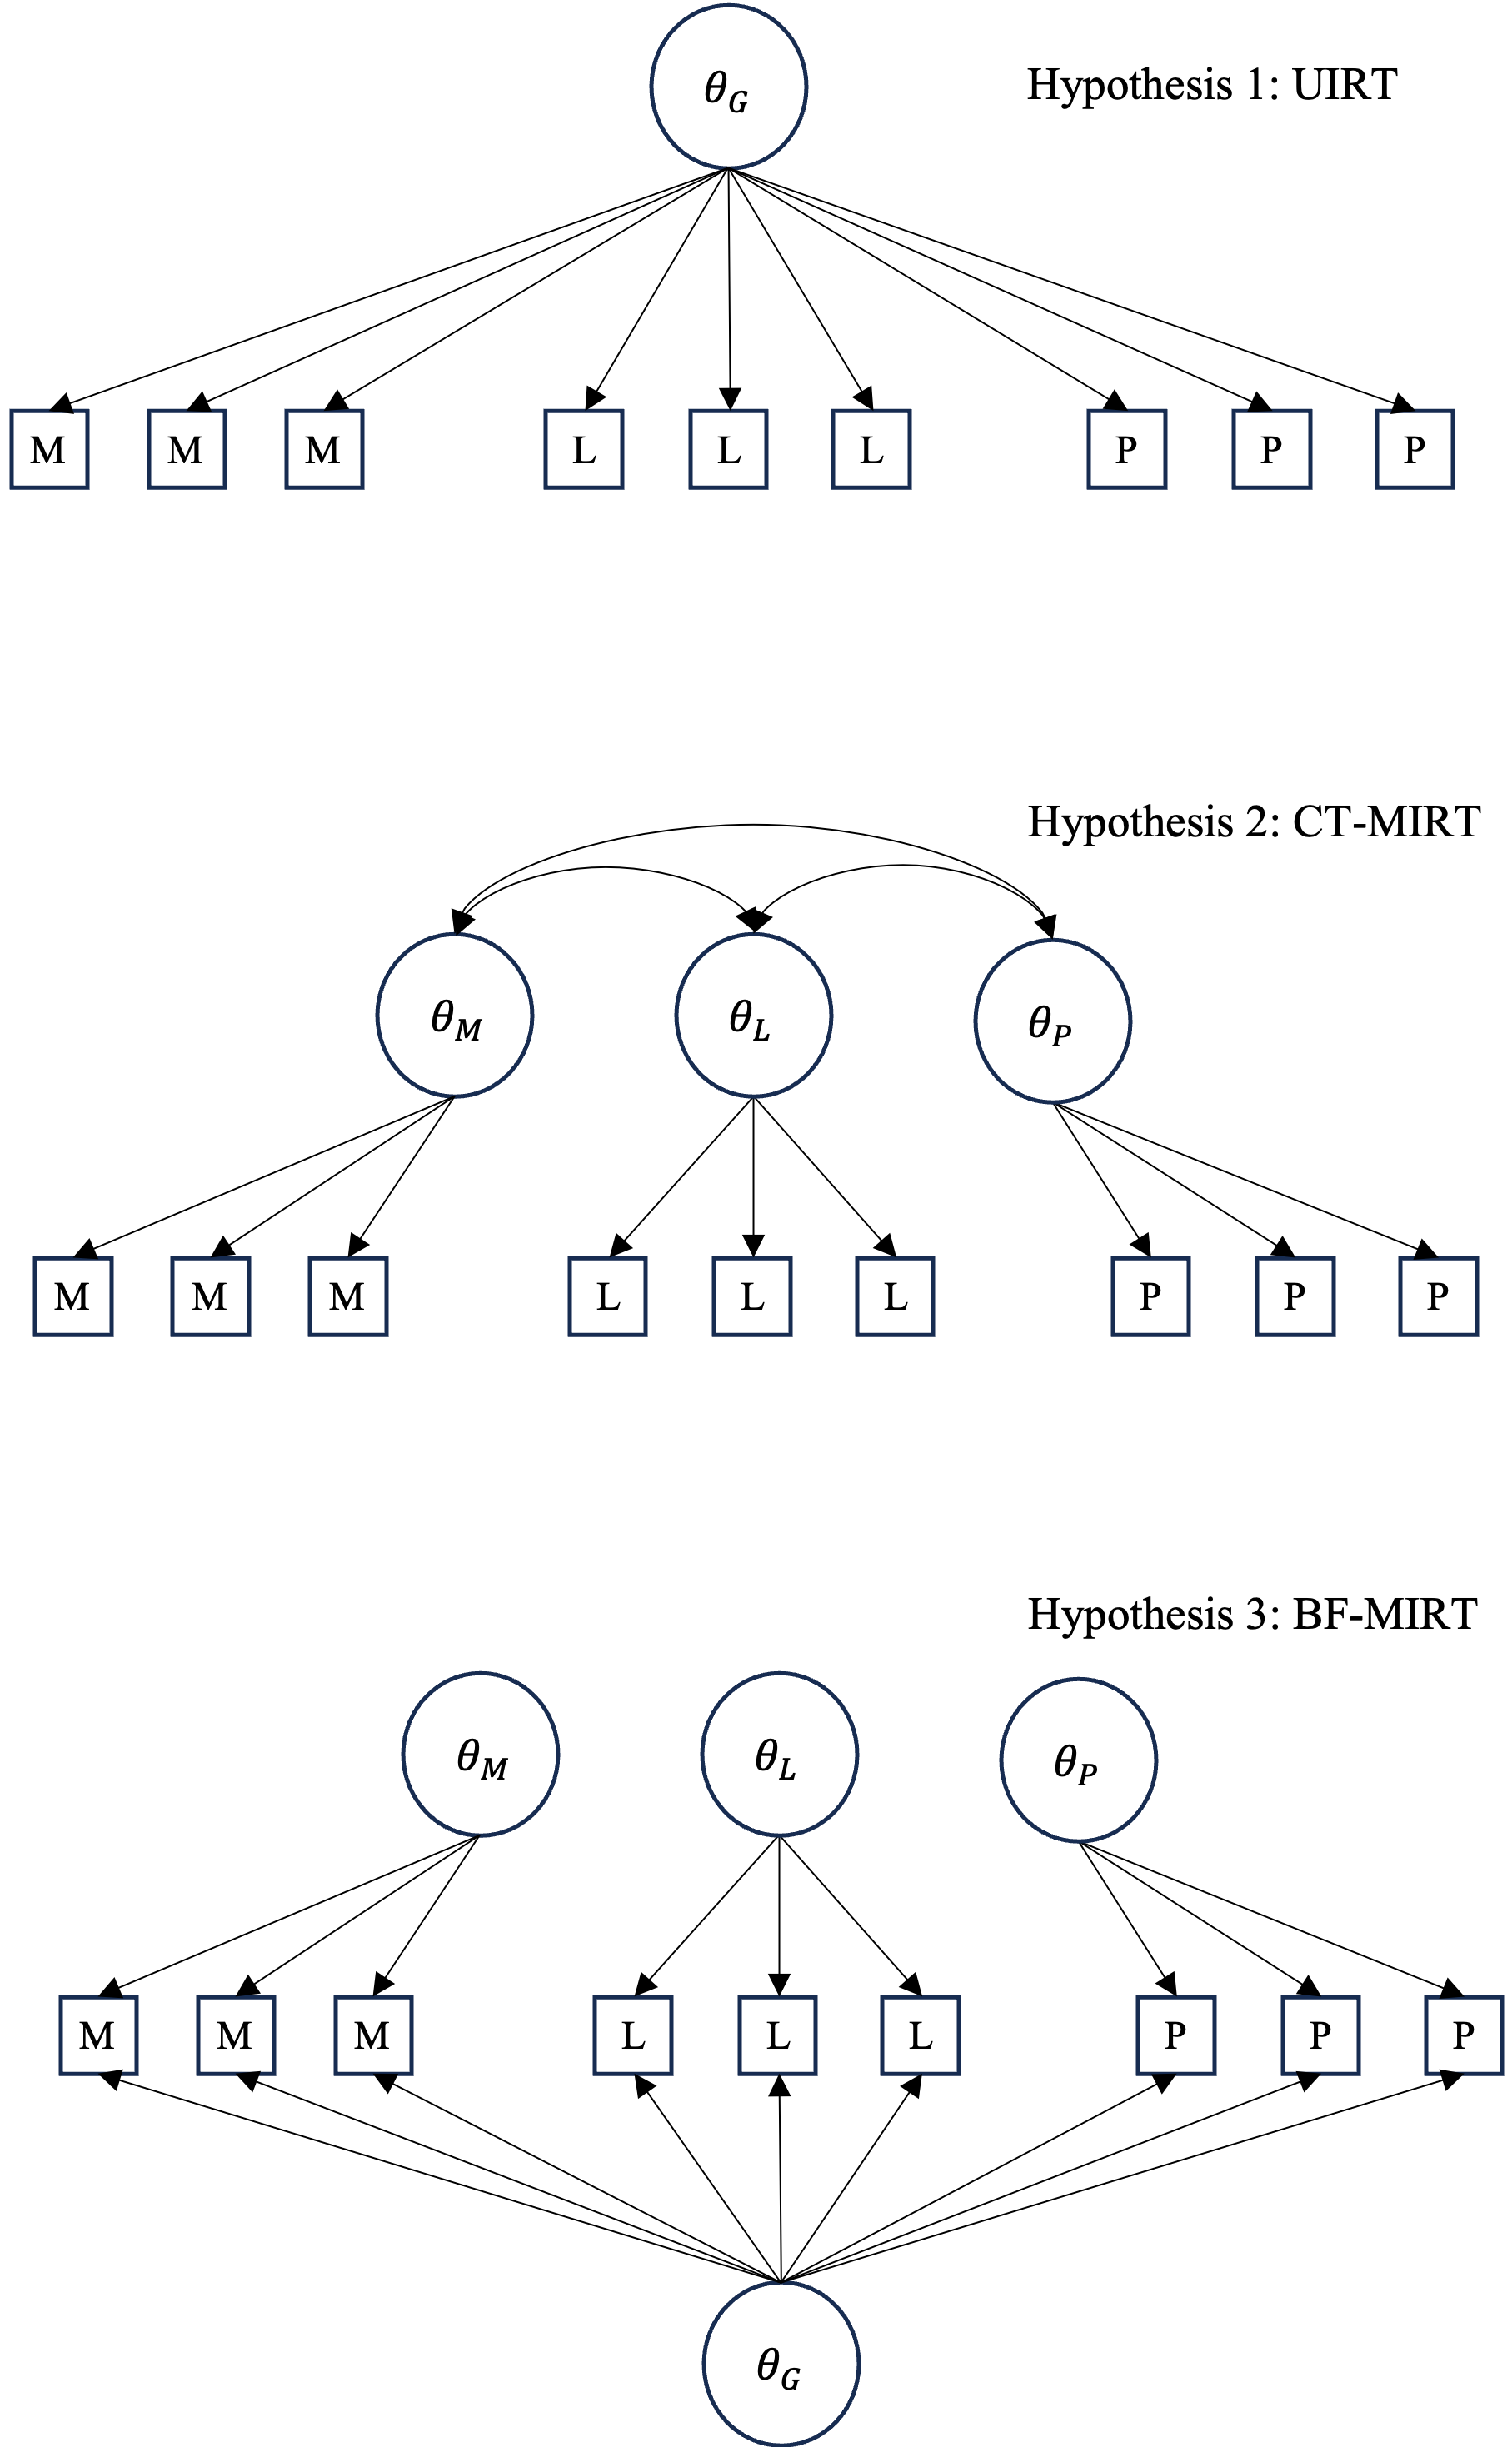
\includegraphics[width=0.7\linewidth,height=\textheight,keepaspectratio]{../figures/fig2.png}

}

\end{figure}%

In the notation below, \(\eta_{pi}\) denotes the linear predictor for
person \(p\) on item \(i\) (mapped to category probabilities by the
ordinal link function), \(\beta_0\) is the fixed intercept, \(\xi_i\) is
item \(i\)'s difficulty, and \(\mathbb{I}_{id}\) is a binary indicator
assigning item \(i\) to dimension \(d \in \{M, L, P\}\).

\emph{Unidimensional.} The simplest assumption is that all items measure
a single continuum of inclusive belief. This implies that teachers'
orientations toward mathematics, learners, and pedagogy vary in concert,
so that a single latent trait \(\theta_p\) suffices:

\[
\eta_{pi} = \beta_0 + \xi_i + \theta_p
\]

\emph{Correlated traits.} According to belief cluster theory (Green,
1971), teachers' beliefs are not monolithic but organised in clusters
that may develop and function semi-independently. Applied to this
instrument, the three subscales may represent distinct yet
interconnected belief clusters, allowing, for instance, a teacher to
hold formalist views of mathematics while still believing most students
can succeed. Each person is then characterised by a vector
\(\boldsymbol{\theta}_p = (\theta_{pM}, \theta_{pL}, \theta_{pP})^\top
\sim \mathcal{N}(\mathbf{0}, \boldsymbol{\Sigma})\) with an unrestricted
covariance matrix:

\[
\eta_{pi} = \beta_0 + \xi_i 
  + \sum_{d \in \{M,L,P\}} \mathbb{I}_{id}\, \theta_{pd}
\]

\emph{Bi-factor.} Belief system theories (Green, 1971; Rokeach, 1968)
further propose that beliefs form hierarchical networks in which some
core beliefs are stable and broadly influential, while others are more
peripheral and context-dependent. Statistically, this implies a
bi-factor structure: a general inclusive belief factor captures the
shared variance across all items, while dimension-specific residual
factors capture variation not explained by the general factor. A general
trait \(\theta_p\) is added alongside orthogonal specific factors
\(\theta_{pd}^{s}\):

\[
\eta_{pi} = \beta_0 + \xi_i + \theta_p 
  + \sum_{d \in \{M,L,P\}} \mathbb{I}_{id}\, \theta_{pd}^{s}
\]

The orthogonality constraint
\(\text{Cov}(\theta_p, \theta_{pd}^{s}) = 0\) is imposed
here.\footnote{It is possible to relax this constraint and estimate
  correlations between the general and specific factors. However, doing
  so introduces identification difficulties, as the model must
  distinguish general-factor variance from correlated specific-factor
  variance using the same set of item responses. With small samples this
  also raises the risk of overfitting, where the additional covariance
  parameters absorb noise rather than capturing meaningful structure.}
Its implementation in brms is discussed in Section 5.2. All three
hypotheses can be combined with any of the ordinal link functions
described in Appendix A; competing combinations are systematically
compared in the workflow.

\subsubsection{Computational setup}\label{computational-setup}

All models were fitted in R using the brms package (Bürkner, 2017),
which interfaces with Stan (Carpenter et al., 2017) for Hamiltonian
Monte Carlo sampling. Each model used 4 chains with 4,000 iterations per
chain (2,000 warmup), yielding 8,000 post-warmup draws for inference.
Weakly informative priors were specified following Bürkner
(\citeproc{ref-burkner2021bayesi}{2021}) : \(\mathcal{N}(0, 3)\) for
person and item random effect standard deviations, \(\mathcal{N}(0, 1)\)
for log-discrimination parameters, and \(\text{LKJ}(2)\) for correlation
matrices in the correlated-traits models.\footnote{The LKJ prior
  (Lewandowski, Kurowicka, \& Joe, 2009) is a distribution over
  correlation matrices. The shape parameter \(\eta\) controls the
  density: \(\eta = 1\) is uniform over all valid correlation matrices;
  \(\eta > 1\) increasingly concentrates density near the identity
  matrix, favouring smaller correlations. We use \(\eta = 2\) as a mild
  regularising choice.} Convergence was assessed by confirming
\(\hat{R} < 1.01\) for all parameters, adequate bulk and tail effective
sample sizes, and no persistent divergent transitions. Additional
sampler settings introduced for complex multidimensional models are
discussed alongside the relevant workflow steps. Complete code is
provided in the companion repository.

\newpage

\section{References}\label{references}

\phantomsection\label{refs}
\begin{CSLReferences}{1}{0}
\bibitem[\citeproctext]{ref-burkner2021bayesi}
Bürkner, P.-C. (2021). Bayesian item response modeling in {R} with brms
and {Stan}. \emph{Journal of Statistical Software}, \emph{100}, 1--54.

\end{CSLReferences}

\newpage

\appendix

\section{Model specifications}\label{apx-models}

This appendix provides detailed mathematical specifications of the
ordinal IRT models used in this study. All models are extensions of IRT
for ordered categorical responses, differing in their link functions,
threshold parameterisations, and discrimination constraints.
Implementation details in brms are provided in the main text and
companion repository.

\subsection{Ordinal Link Functions and Threshold
Parameterisations}\label{ordinal-link-functions-and-threshold-parameterisations}

\subsubsection{Rating Scale Model (RSM)}\label{rating-scale-model-rsm}

The RSM uses the adjacent-category logit link with shared thresholds.
The probability of person \(p\) responding in category \(c\)
(\(c = 1, \ldots, C\)) to item \(i\) is:

\[
P(Y_{pi} = c) = \frac{\exp \sum_{j=1}^{c} (\theta_p + \xi_i - \tau_j)}{\sum_{r=1}^{C} \exp \sum_{j=1}^{r} (\theta_p + \xi_i - \tau_j)}
\]

where \(\theta_p\) is the latent trait of person \(p\), \(\xi_i\) is the
item-specific location (random intercept; more negative = harder to
endorse), and \(\tau_j\) is the \(j\)-th threshold parameter. A key
constraint of the RSM is that thresholds \(\tau_j\) are shared across
all items, assuming equal category spacing across the instrument.

\subsubsection{Generalised Rating Scale Model
(GRSM)}\label{generalised-rating-scale-model-grsm}

Introducing item-specific discrimination parameters \(\alpha_i\) to the
RSM yields the GRSM:

\[
P(Y_{pi} = c) = \frac{\exp \sum_{j=1}^{c} \alpha_i(\theta_p + \xi_i - \tau_j)}{\sum_{r=1}^{C} \exp \sum_{j=1}^{r} \alpha_i(\theta_p + \xi_i - \tau_j)}
\]

Higher \(\alpha_i\) values indicate items that more sharply
differentiate between respondents at different trait levels. Thresholds
remain shared across items.

\subsubsection{Generalised Partial Credit Model
(GPCM)}\label{generalised-partial-credit-model-gpcm}

The GPCM combines item-specific discrimination with item-specific
thresholds \(\tau_{i,j}\):

\[
P(Y_{pi} = c) = \frac{\exp \sum_{j=1}^{c} \alpha_i(\theta_p + \xi_i - \tau_{i,j})}{\sum_{r=1}^{C} \exp \sum_{j=1}^{r} \alpha_i(\theta_p + \xi_i - \tau_{i,j})}
\]

Unlike the GRSM, which constrains all items to share the same threshold
spacing, the GPCM allows each item to have its own set of threshold
parameters. This provides the most flexible parameterisation within the
adjacent-category family, but requires estimating substantially more
parameters, which can compromise stability with small samples. \#\#\#
Graded Response Model (GRM)

The GRM uses the cumulative logit link rather than the adjacent-category
logit. In its general form (Samejima, 2016), the GRM allows fully
item-specific thresholds. The implementation used in this study is a
constrained variant in which threshold spacing is shared across items,
with item differences captured through a location parameter \(\xi_i\)
that shifts all thresholds equally. The probability of responding in
category \(c\) is defined as:

\[
P(Y_{pi} = c) = F\!\left(\alpha_i(\eta_{pi} - \tau_{c-1})\right) - F\!\left(\alpha_i(\eta_{pi} - \tau_c)\right)
\]

where \(\eta_{pi} = \theta_p + \xi_i\) is the person-by-item location,
\(F(x) = \frac{1}{1 + \exp(-x)}\) is the logistic CDF, \(\alpha_i\) is
item discrimination, and the thresholds are ordered:
\(\tau_1 < \cdots < \tau_{C-1}\), with boundary conditions
\(\tau_0 = -\infty\) and \(\tau_C = +\infty\). The thresholds \(\tau_c\)
are shared population-level parameters; item \(i\)'s effective
thresholds are \(\tau_c - \xi_i\), preserving equal inter-threshold
spacing across items.

The GRM directly models the cumulative probability \(P(Y_{pi} \geq c)\),
in contrast to the adjacent-category models which model the odds of each
category relative to its neighbour.

\newpage

\subsubsection{Summary of Model
Families}\label{summary-of-model-families}

\begingroup
\fontsize{10.5pt}{12.6pt}\selectfont

\begin{table}

{\caption{{Summary of ordinal IRT model families used in this study.
RSM, GRSM, and GRM share threshold spacing across items; item
differences enter only through the location parameter \(\xi_i\). GPCM
allows fully item-specific thresholds. The generalised forms (GRSM,
GPCM, GRM) estimate item-specific discrimination.}{\label{tbl-models}}}
\vspace{-20pt}}

\begin{longtable}[]{@{}
  >{\raggedright\arraybackslash}p{(\linewidth - 6\tabcolsep) * \real{0.1500}}
  >{\raggedright\arraybackslash}p{(\linewidth - 6\tabcolsep) * \real{0.2500}}
  >{\raggedright\arraybackslash}p{(\linewidth - 6\tabcolsep) * \real{0.3000}}
  >{\raggedright\arraybackslash}p{(\linewidth - 6\tabcolsep) * \real{0.3000}}@{}}
\toprule\noalign{}
\begin{minipage}[b]{\linewidth}\raggedright
Model
\end{minipage} & \begin{minipage}[b]{\linewidth}\raggedright
Link
\end{minipage} & \begin{minipage}[b]{\linewidth}\raggedright
Thresholds
\end{minipage} & \begin{minipage}[b]{\linewidth}\raggedright
Discrimination
\end{minipage} \\
\midrule\noalign{}
\endhead
\bottomrule\noalign{}
\endlastfoot
RSM & Adjacent-category & Shared & Equal (\(\alpha = 1\)) \\
GRSM & Adjacent-category & Shared & Item-specific \\
GPCM & Adjacent-category & Item-specific & Item-specific \\
GRM & Cumulative & Shared (equal spacing) & Item-specific \\
\end{longtable}

\end{table}

\endgroup

\subsection{Dimensional Structures}\label{dimensional-structures}

All models in this study are implemented as generalised linear mixed
models (GLMMs) in brms, following the framework described in De Boeck et
al.~(2011) and Bürkner (2021).

\subsubsection{Unidimensional IRT}\label{unidimensional-irt}

\[
\eta_{pi} = \beta_0 + \xi_i + \theta_p
\]

where \(\beta_0\) is the fixed intercept,
\(\xi_i \sim \mathcal{N}(0, \sigma^2_{\text{item}})\) is the
item-specific random intercept, and
\(\theta_p \sim \mathcal{N}(0, \sigma^2_{\theta})\) is the
person-specific random effect.

\subsubsection{Correlated-Traits MIRT
(CT-MIRT)}\label{correlated-traits-mirt-ct-mirt}

Each person \(p\) has a vector of dimension-specific traits:

\[
\boldsymbol{\theta}_p = (\theta_{pM}, \theta_{pL}, \theta_{pP})^\top \sim \mathcal{N}(\mathbf{0}, \boldsymbol{\Sigma})
\]

where \(\boldsymbol{\Sigma}\) is a \(3 \times 3\) covariance matrix. The
linear predictor is:

\[
\eta_{pi} = \beta_0 + \xi_i + \sum_{d \in \{M, L, P\}} \mathbb{I}_{id}\, \theta_{pd}
\]

where \(\mathbb{I}_{id} = 1\) if item \(i\) belongs to dimension \(d\)
and 0 otherwise (each item loads on exactly one dimension). The
unrestricted covariance matrix \(\boldsymbol{\Sigma}\) allows the three
latent dimensions to correlate freely, reflecting the possibility that
the dimensions are distinct but related constructs.

\subsubsection{Bi-Factor MIRT (BF-MIRT)}\label{bi-factor-mirt-bf-mirt}

A general factor \(\theta_p\) is added alongside dimension-specific
factors \(\theta_{pd}^{s}\):

\[
\eta_{pi} = \beta_0 + \xi_i + \theta_p + \sum_{d \in \{M, L, P\}} \mathbb{I}_{id}\, \theta_{pd}^{s}
\]

where \(\theta_p \sim \mathcal{N}(0, \sigma^2_{\theta})\) and
\(\theta_{pd}^{s} \sim \mathcal{N}(0, \sigma^2_{d})\). The general and
specific factors are constrained to be orthogonal:

\[
\text{Cov}(\theta_p, \theta_{pd}^{s}) = 0 \quad \forall\, d
\]

This constraint ensures that the specific factors capture only residual
variation within each dimension after accounting for the general factor.
The distinction from CT-MIRT is structural: the correlated-traits model
permits free correlations among dimension-specific traits but includes
no general factor, whereas the bi-factor model decomposes variance into
a general component shared across all items and orthogonal
dimension-specific residuals.

\newpage

\subsection{Prior Distributions}\label{prior-distributions}

Weakly informative priors are used throughout, following recommendations
in Bürkner (2021):

\begingroup
\fontsize{10.5pt}{12.6pt}\selectfont

\begin{table}

{\caption{{Prior distributions for all model
parameters.}{\label{tbl-priors}}}
\vspace{-20pt}}

\begin{longtable}[]{@{}
  >{\raggedright\arraybackslash}p{(\linewidth - 4\tabcolsep) * \real{0.3500}}
  >{\raggedright\arraybackslash}p{(\linewidth - 4\tabcolsep) * \real{0.2000}}
  >{\raggedright\arraybackslash}p{(\linewidth - 4\tabcolsep) * \real{0.4500}}@{}}
\toprule\noalign{}
\begin{minipage}[b]{\linewidth}\raggedright
Parameter
\end{minipage} & \begin{minipage}[b]{\linewidth}\raggedright
Prior
\end{minipage} & \begin{minipage}[b]{\linewidth}\raggedright
Rationale
\end{minipage} \\
\midrule\noalign{}
\endhead
\bottomrule\noalign{}
\endlastfoot
Person and item SDs (\(\sigma_\theta\), \(\sigma_{\text{item}}\)) &
\(\mathcal{N}(0, 3)\) & Half-normal (truncated at 0); allows substantial
variation while regularising. \\
Log-discrimination SD & \(\mathcal{N}(0, 1)\) & Covers discrimination
values roughly in \([0.14, 7.4]\). \\
Correlation matrix (CT-MIRT) & \(\text{LKJ}(2)\) & Mildly favours
smaller correlations; \(\eta > 1\) concentrates density near the
identity matrix. \\
\end{longtable}

\end{table}

\endgroup

\newpage

\section{Instrument items}\label{apx-items}

Teachers were asked to report their endorsement of each statement on a
5-point Likert scale from ``strongly disagree'' (1) to ``strongly
agree'' (5). Items ending with \texttt{\_r} are reverse-coded: responses
are recoded prior to analysis so that higher scores consistently reflect
stronger endorsement of inclusive and equity-oriented beliefs.

\subsection{Bm: Beliefs About Mathematics (8
Items)}\label{bm-beliefs-about-mathematics-8-items}

\begingroup
\fontsize{10.5pt}{12.6pt}\selectfont

\begin{table}

{\caption{{Beliefs about mathematics items.}{\label{tbl-item-bm}}}
\vspace{-20pt}}

\begin{longtable}[]{@{}
  >{\raggedright\arraybackslash}p{(\linewidth - 2\tabcolsep) * \real{0.1500}}
  >{\raggedright\arraybackslash}p{(\linewidth - 2\tabcolsep) * \real{0.8500}}@{}}
\toprule\noalign{}
\begin{minipage}[b]{\linewidth}\raggedright
Item
\end{minipage} & \begin{minipage}[b]{\linewidth}\raggedright
Statement
\end{minipage} \\
\midrule\noalign{}
\endhead
\bottomrule\noalign{}
\endlastfoot
Bm\_1\_r & Mathematics is a collection of rules and procedures. \\
Bm\_2\_r & Mathematics involves remembering and applying definitions,
formulas, mathematical facts and procedures. \\
Bm\_3\_r & To do mathematics requires much practice of correct
application of routines. \\
Bm\_4\_r & When solving mathematical tasks you need to know the correct
procedure in advance. \\
Bm\_5 & Mathematics involves creativity and new ideas. \\
Bm\_6 & Many aspects of mathematics have practical relevance. \\
Bm\_7 & Mathematics helps solve everyday problems and tasks. \\
Bm\_8 & In mathematics many things can be discovered and tried out by
oneself. \\
\end{longtable}

\end{table}

\emph{Note.} Items Bm\_1\_r through Bm\_4\_r were removed during the
workflow due to poor psychometric properties. The final model was fitted
on the remaining 20 items. \endgroup

\newpage

\subsection{Bl: Beliefs About Learners (11
Items)}\label{bl-beliefs-about-learners-11-items}

\begingroup
\fontsize{10.5pt}{12.6pt}\selectfont

\begin{table}

{\caption{{Beliefs about learners items.}{\label{tbl-item-bl}}}
\vspace{-20pt}}

\begin{longtable}[]{@{}
  >{\raggedright\arraybackslash}p{(\linewidth - 2\tabcolsep) * \real{0.1500}}
  >{\raggedright\arraybackslash}p{(\linewidth - 2\tabcolsep) * \real{0.8500}}@{}}
\toprule\noalign{}
\begin{minipage}[b]{\linewidth}\raggedright
Item
\end{minipage} & \begin{minipage}[b]{\linewidth}\raggedright
Statement
\end{minipage} \\
\midrule\noalign{}
\endhead
\bottomrule\noalign{}
\endlastfoot
Bl\_1\_r & Students must be able to solve mathematics problems
quickly. \\
Bl\_2 & Students must be able to understand why the answer is
correct. \\
Bl\_3\_r & Students learn mathematics best by attending to the teacher's
standard explanations. \\
Bl\_4\_r & For students, non-standard procedures can interfere with
learning the correct procedure. \\
Bl\_5 & Students can figure out a way to solve mathematical problems
without a teacher's help. \\
Bl\_6\_r & Only the more able students can participate in mathematics
activities. \\
Bl\_7\_r & To be good at mathematics one needs to be talented. \\
Bl\_8\_r & Among other forms of talent, mathematical talent is
relatively fixed. \\
Bl\_9\_r & Boys tend to be more talented in mathematics than girls. \\
Bl\_10\_r & Attention to mathematically weak students can interfere with
the learning experience of other students. \\
Bl\_11\_r & Attention to mathematically talented students can interfere
with the learning experience of other students. \\
\end{longtable}

\end{table}

\endgroup

\subsection{Bp: Beliefs About Pedagogy (5
Items)}\label{bp-beliefs-about-pedagogy-5-items}

\begingroup
\fontsize{10.5pt}{12.6pt}\selectfont

\begin{table}

{\caption{{Beliefs about pedagogy items.}{\label{tbl-item-bp}}}
\vspace{-20pt}}

\begin{longtable}[]{@{}
  >{\raggedright\arraybackslash}p{(\linewidth - 2\tabcolsep) * \real{0.1500}}
  >{\raggedright\arraybackslash}p{(\linewidth - 2\tabcolsep) * \real{0.8500}}@{}}
\toprule\noalign{}
\begin{minipage}[b]{\linewidth}\raggedright
Item
\end{minipage} & \begin{minipage}[b]{\linewidth}\raggedright
Statement
\end{minipage} \\
\midrule\noalign{}
\endhead
\bottomrule\noalign{}
\endlastfoot
Bp\_1\_r & Innovative pedagogy (e.g., project-based learning, flipped
classroom) is not worth the time and expense. \\
Bp\_2\_r & Innovative pedagogy (e.g., project-based learning, flipped
classroom) should only play a minor, supplementary role in the
mathematics classroom. \\
Bp\_3 & I'm continuously seeking better ways to teach mathematics. \\
Bp\_4 & Teachers should help students using mathematics to critically
analyse the world. \\
Bp\_5 & Discussion of social issues should be involved in the maths
classroom. \\
\end{longtable}

\end{table}

\endgroup






\end{document}
